\section{Background}

The eduROV project started as an idea at Trondheim Maker Faire in 2014. From there on it has been developed into a \emph{"functioning Open-Source ROV project at a new level of affordability."}\footnote{\url{https://www.edurov.no/}}. The project is managed by Norwegian University of Science and Technology (NTNU) and in specific the \emph{engage} project by Centre for Engaged Education through Entrepreneurship. It aims to let hobbyists, enthusiasts and schools to create a simple, affordable and open-source underwater ROV. From the 25th of June until July the 6th a summer school will be hosted at NTNU where high school student will build and test this ROV.

I, the author of this thesis, had participated in a course where I developed a similar ROV. In Desember 2017 I joined the project to improve the software which was used to control and display information from the ROV. There was three main areas that needed software improvements. First, the video latency was almost 800ms when using a cabled ethernet connection. Secondly, the software provided little to none user customization. Lastly, the user interface was not very attractive and had few features.

The ROV consisted of a Raspberry Pi 3 Model B+ (RPi) and an Arduino Micro. The Arduino was responsible for reading sensor values and controlling motors. The RPi had multiple tasks, it communicated with the Arduino by reading sensor values and sending motor speed commands. In addition, it captured video from the RPi camera module and displayed this to the user. Lastly, it processed user input from the operator and forwarded these commands to the Arduino.

On the RPi a python program using the \emph{Pygame}\footnote{\url{pygame}} package was running. This is an open source package created for making games, but it can also be used to display video feed and read user input. When initiated, this program would display a window on the RPi. \emph{RealVNC}, a software for remote desktop viewing was then used to display this window on the remote computer used for control. \figref{edurovOld} shows this user interface (UI). The software did not require any installation, instead the correct files had to be copied from a GitHub repository.

\begin{figure}[h!]
    \centering
    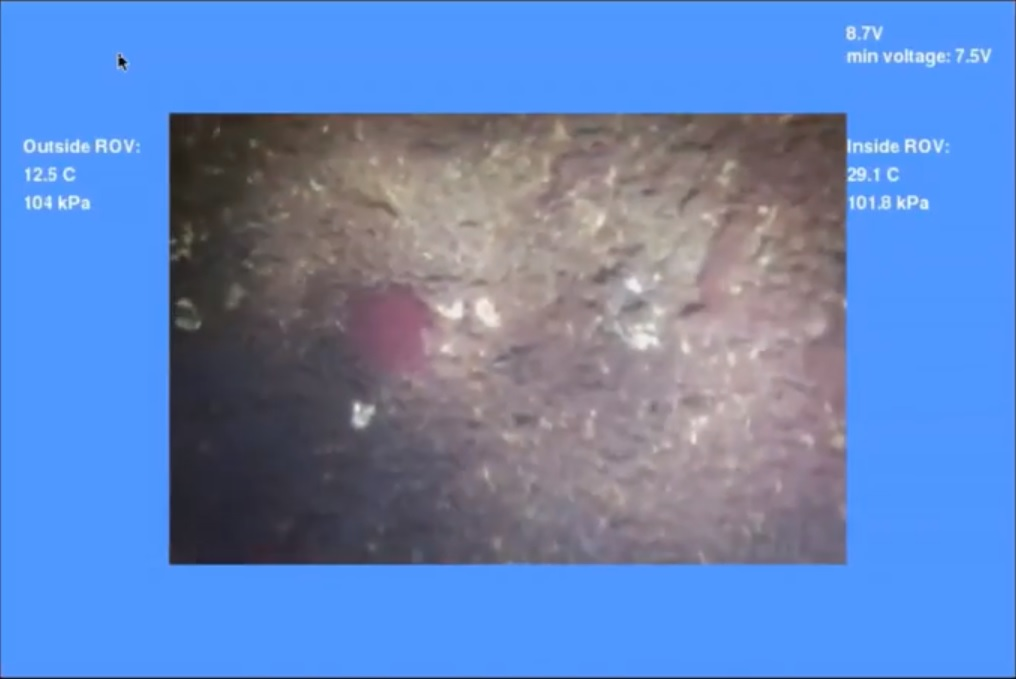
\includegraphics[width=0.8\textwidth]{edurovOld}
    \caption{User interface for the original eduROV.}
    \label{edurovOld}
\end{figure}

Some goals were then set for my contribution to the project:

\begin{itemize}
\item Reduce the video latency as much as possible while still having the possibility for high resolution images.

\item Streamline the installation process, i.e. remove the need for visiting any website or manually coping files.

\item Remove the need for any third party applications, that would mean removing the RealVNC dependency for video transfer.

\item Increase customization while still maintaining a high level application programming interface (API).

\item Make the UI more attractive, include more UI features without overwhelming the operator.
\end{itemize}

\section{Current alternatives}

There exists a wealth of software's created for operating ROV's. This discussion will be limited to those that are open source and created in Python. The most well known and probably most used is the \emph{Robot Operating System} (ROS)\footnote{\url{http://www.ros.org/}} which is ported to python as a client library called \emph{rospy}\footnote{\url{http://wiki.ros.org/rospy}}. Although a powerful framework, it does not not suit the needs of this project. Originally written C++, ROS was originally not created for python. This means that the documentation is mostly in C++ and for anyone who wanted to customize the eduROV software in the future would have learn ROS in addition to python. It was decided that making ROS fit the needs of the eduROV would require more time and be limiting to the development, in comparison to creating a tailored software from scratch.

There is also something called \emph{GoPiGo}\footnote{\url{https://www.dexterindustries.com/gopigo3/}}. This started as a Kickstarter project and is now a hardware / software project that you can buy online. It provides robot communication with video feed, but the software seems to created specifically for the robots they sell. The software is also not created as a package meant for other users to build on.

In summary, there wasn't really any good software alternatives for the eduROV project. Actually, I was not able to find any python packages created for ROV communication with video support built in. There are many guides on the internet that will walk you through how to create this, but the whole process can be really intimidating for people with limited experience. In addition, many of the guides online require you to install multiple software's and download files from additional places. Not very user friendly. Also, in the guides online they often control ROV's by pushing buttons on a screen, not by keyboard input. Lastly, they contain limited to none documentation.

\section{Development}

All popular and well known packages in the python community is developed inline with the \emph{Python Packaging User Guide}\footnote{\url{https://packaging.python.org/}}. This guide establishes multiple rules on how packages should be developed and distributed. In comparison it is always possible to upload code to a remote repository and ask people to download it from there. But there are many good reasons why any serious actors use this method. By distributing the code through the \emph{Python Package Index}, anyone can install the package by running \texttt{"pip install edurov"} in a command terminal. No need to visit any websites or copy any files. This command will download install the required files automatically. Second reason is that this greatly simplifies the process of documentation. By creating special files as stated by the guidelines, a separate website with all the documentation is created and uploaded automatically. It also specifies rules for a versioning scheme. This let's the developer create alpha, beta, release candidates and deployment versions of the software. It makes it easy to make sure that everything is tested properly before it get's publicly available.

Git version control was used throughout the project. All the code was uploaded to the remote repository at \url{https://github.com/trolllabs/eduROV}. Git branches was used for rapid prototyping of different ideas. This meant that different approaches were developed concurrently in each their branch. They were then removed one after another as it became clear that the approach did not meet the requirements.

In the first phase of the development which contained very different branches, two main methods were tested. The first method was based upon the \emph{pygame} package. It required the operator to install python and the eduROV package on both the ROV and the controlling computer itself. When the software was started a program window would pop up on the controlling computer and display the video feed. Any customization to the features and UI would require the user to learn pygame since all the graphics are created using the pygame API. The original software used pygame, only difference is that it used RealVNC for transmission.

The second method was based upon a very different approach. This method started a web server on the ROV which could then be viewed on any device connected to the same network as the ROV. This meant that the operator would not have to install any software on his or hers computer. It also meant that the UI would be created using html and css instead of pure python. This approach were chosen for the new eduROV package. It would completely remove the need to install anything on the operator computer. It would make it possible to view the video stream at multiple devices at the same time. In addition, web browsers has been around for a very long time and much effort has been spent on making them as efficient and flexible as possible. By using the browser as a medium it's possible to take advantage of this. Some high schools also have web development and html as part of their curriculum. By basing the the eduROV package on a web server framework it becomes possible to let the operator customize the UI with their knowledge of html and css.

When the main method were chosen, future development were guided by \emph{GitHub issues workflow}. \figref{issues} shows a section of the \emph{issues} page on GitHub.

\begin{figure}[h!]
    \centering
    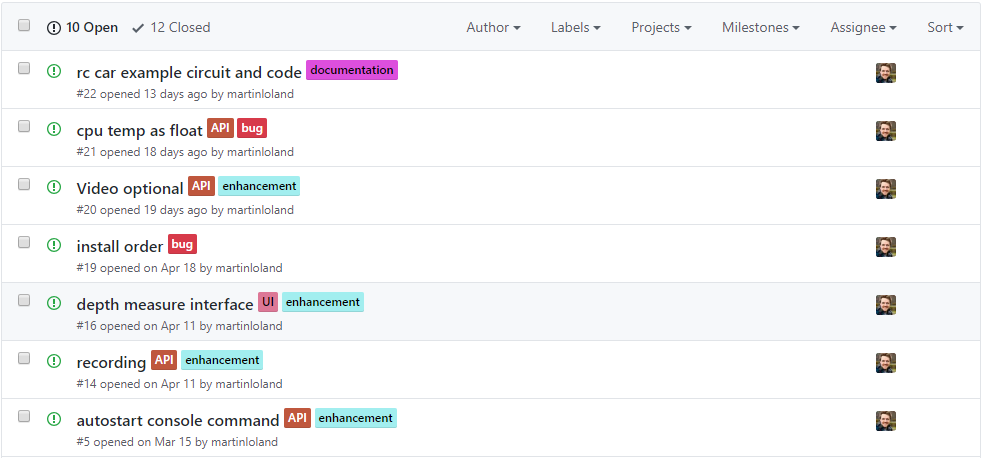
\includegraphics[width=\textwidth]{issues}
    \caption{GitHub issues overview.}
    \label{issues}
\end{figure}

\section{Architecture}
\todo[inline]{
- socket protocols / Pyro4

- HTTP Webserver, ethernet and wifi

- different processes / Parallelism

- camera capture
}

\missingfigure{Graphics showing the architecture, hardware and software}

\section{Graphical user interface}
\todo[inline]{
- html and js

- customizable

- in the context of engage

- attitude
}

\citep{Chen2007} "Attitude (i.e., pitch and roll) of a robotic vehicle may be easy to reference when there are other familiar objects (e.g., horizon, buildings, trees, etc.) in the re- mote environment.However, if those reference points are absent and the on-board cameras are fixed, operators sometimes find it surprisingly hard to accurately assess the attitude of their robotic vehicles."

\citep{Wang2004} Gravity-Referenced Attitude Display for Teleoperation of Mobile Robots

\citep{Chen2007} "The ideal view depends on the task; overall awareness and pattern recognition are optimized by exocentric views whereas the immediate environment is often viewed better egocentrically."
"overlaying information on video feed can potentially lead to cognitive tunneling"

\missingfigure{Image showing the GUI of the eduROV submersible}

\section{Application programming interface}

\todo[inline]{
- WebMethod
}

\section{Performance}

\missingfigure{Image showing the video latencies at different resolutions}

\section{Documentation}

\todo[inline]{
- Read the docs with git

- Restructured text

- Autodoc with git

- Examples
}

\missingfigure{example code of how the documentation is written}

\missingfigure{example image of how this text is shown in the web browser}

\section{Novelty features}

\todo[inline]{
- main features from docs

- what does it do better than the competition

- future work

- websockets

- flask?
}